\documentclass[]{article}

\usepackage[utf8]{inputenc}
\usepackage{amsmath}
\usepackage{amssymb}
\usepackage{amsthm}
\usepackage{amsfonts}
\usepackage{graphicx}
\usepackage{capt-of}
\usepackage{listings}
\usepackage{siunitx}
\usepackage[section]{placeins}
\usepackage{multicol}
\usepackage[a4paper, portrait, margin=1in]{geometry}
\usepackage{float}
\usepackage{caption}
\usepackage{subcaption}
\usepackage{xcolor}

% Solarized colour scheme for listings
\definecolor{solarized@base03}{HTML}{002B36}
\definecolor{solarized@base02}{HTML}{073642}
\definecolor{solarized@base01}{HTML}{586e75}
\definecolor{solarized@base00}{HTML}{657b83}
\definecolor{solarized@base0}{HTML}{839496}
\definecolor{solarized@base1}{HTML}{93a1a1}
\definecolor{solarized@base2}{HTML}{EEE8D5}
\definecolor{solarized@base3}{HTML}{FDF6E3}
\definecolor{solarized@yellow}{HTML}{B58900}
\definecolor{solarized@orange}{HTML}{CB4B16}
\definecolor{solarized@red}{HTML}{DC322F}
\definecolor{solarized@magenta}{HTML}{D33682}
\definecolor{solarized@violet}{HTML}{6C71C4}
\definecolor{solarized@blue}{HTML}{268BD2}
\definecolor{solarized@cyan}{HTML}{2AA198}
\definecolor{solarized@green}{HTML}{859900}

\lstset{language=C++,
        basicstyle=\footnotesize\ttfamily,
        numbers=left,
        numberstyle=\footnotesize,
        tabsize=2,
        breaklines=true,
        escapeinside={@}{@},
        numberstyle=\tiny\color{solarized@base01},
        keywordstyle=\color{solarized@green},
        stringstyle=\color{solarized@cyan}\ttfamily,
        identifierstyle=\color{solarized@blue},
        commentstyle=\color{solarized@base01},
        emphstyle=\color{solarized@red},
        frame=single,
        rulecolor=\color{solarized@base2},
        rulesepcolor=\color{solarized@base2},
        showstringspaces=false
}



% Oppgavenummerering %
\renewcommand\thesection{Task \arabic{section}}
\renewcommand\thesubsection{\alph{subsection})}
\renewcommand\thesubsubsection{\alph{subsection}.\alph{subsubsection})}

% Bevis
\newcommand\TombStone{\rule{.5em}{.5em}}
\renewcommand\qedsymbol{\TombStone}

\title{\Huge{Assignment 3} \\ \Large{TDT4195 – Visual Computing Fundamentals}}
\author{Sigurd Totland | MTTK}

\begin{document}
\maketitle
\begin{multicols}{2}
\section{}
\subsection{}
We begin by simply creating a \texttt{Mesh} object from \texttt{lunarsurface.obj} and sending the vertex, colour, and index vectors into the \texttt{createVAO} function. As expected, the lunar surface renders correctly, albeit without any colors at this time, so it is completely white as shown in figure \ref{fig:white-surface} below.
\begin{figure}[H]
\centering

\includegraphics[width=0.5\columnwidth]{white-surface}
\caption{Lunar surface without any coloring}
\label{fig:white-surface}
\end{figure}

\setcounter{subsection}{2}
\subsection{}
In this task and the previous, we add a third VBO to hold the normals and pass these values through the vertex shader into the fragment shader. Setting the fragment color equal to the x, y, and z components of each normal vector yields a predominantly green surface as shown in figure \ref{fig:green-surface} below.
\begin{figure}[H]
\centering
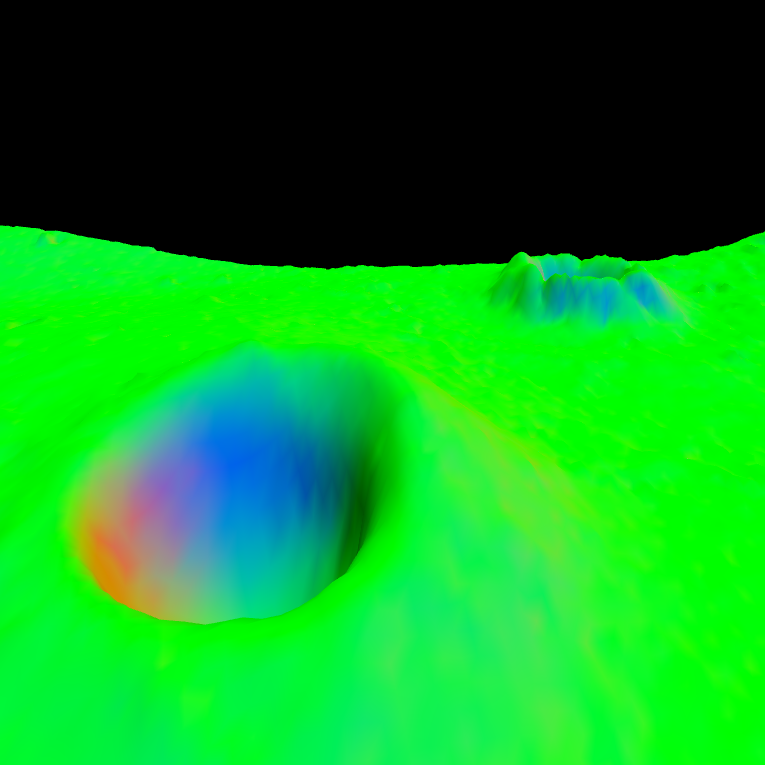
\includegraphics[width=0.5\columnwidth]{green-surface}
\caption{Lunar surface colored by directly inserting the surface normal values}
\label{fig:green-surface}
\end{figure}
We notice how green color corresponds to upward pointing normals, whereas red and blue are for more sideways surfaces.

\subsection{}
Inserting the Lambertian illumination model,
\begin{equation}\begin{aligned}
\text{color} * \max(0, \hat{\mathbf{n}} \cdot (- \hat{\mathbf{l}})),
\end{aligned}\end{equation}
where $\hat{\mathbf{n}}$ is the surface normal and $\hat{\mathbf{l}}$ is the normalized lighting direction the surface becomes a \textit{Lambertian surface}. Coloring the surface a pure white results in the following (quite convincing) scene, clearly showing that the surface is indeed lit. (Figure \ref{fig:lambert-surface}).
\begin{figure}[H]
\centering
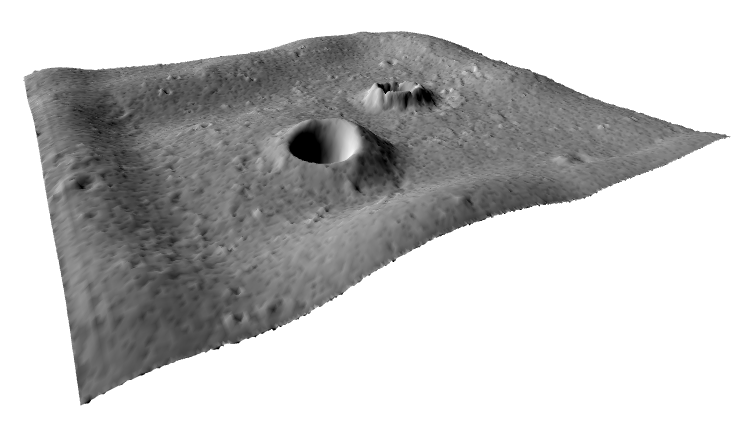
\includegraphics[width=0.5\columnwidth]{lambert-surface}
\caption{Lunar surface with Lambertian shading}
\label{fig:lambert-surface}
\end{figure}
\section{}
\setcounter{subsection}{2}
\subsection{}
We define the scene graph illustrated in figure \ref{fig:scene-graph}.
\begin{figure}[H]
\centering
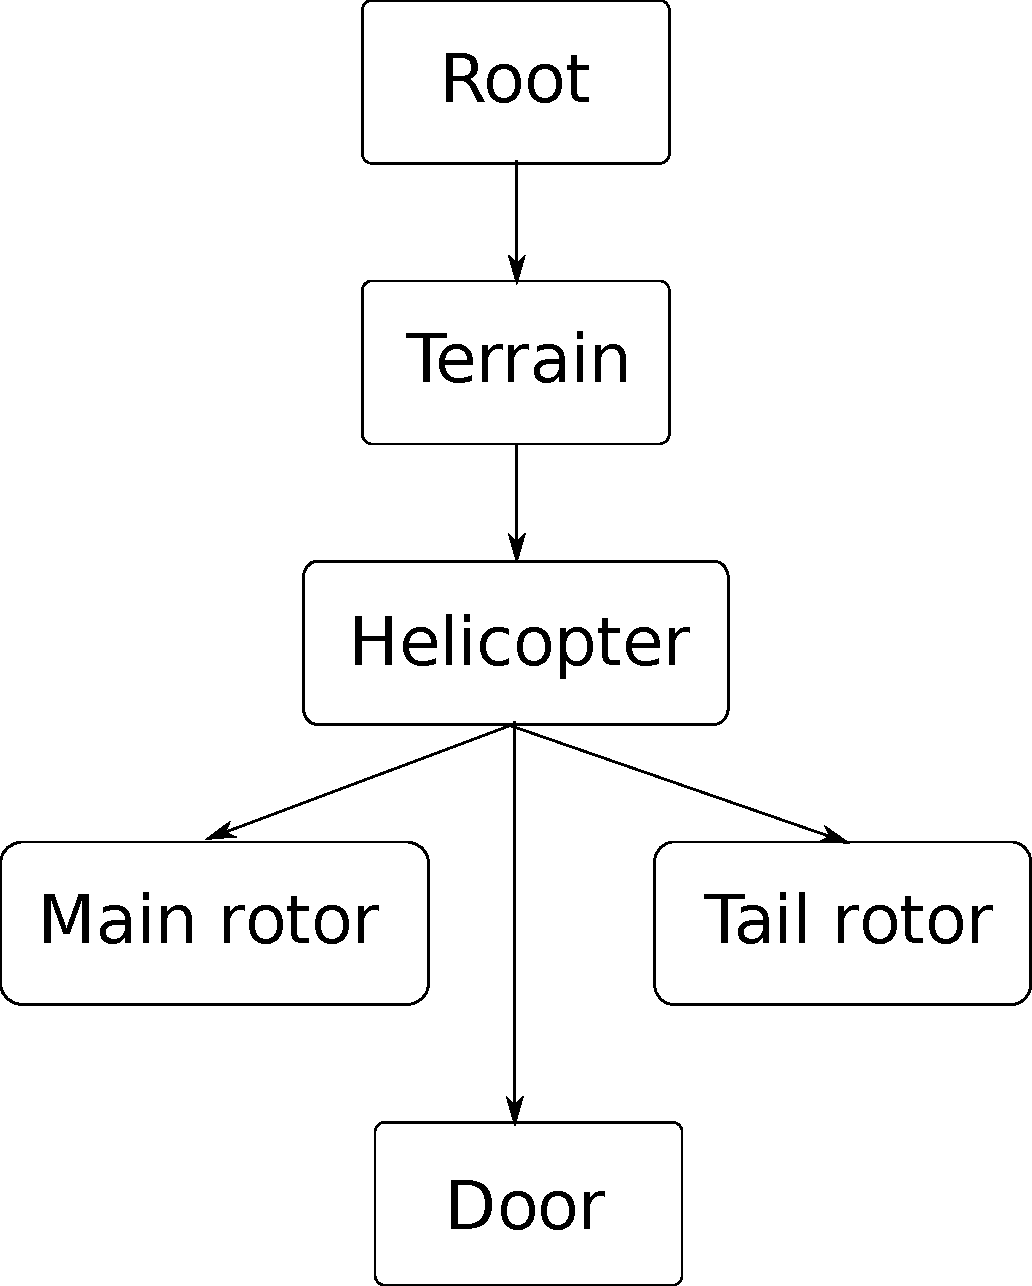
\includegraphics[width=0.5\columnwidth]{scenegraph}
\caption{Scene graph}
\label{fig:scene-graph}
\end{figure}
This graph, when drawn using a basic pre-order recursive draw method yields the physics defying helicopter shown in figure \ref{fig:chopper} below.

\begin{figure}[H]
\centering
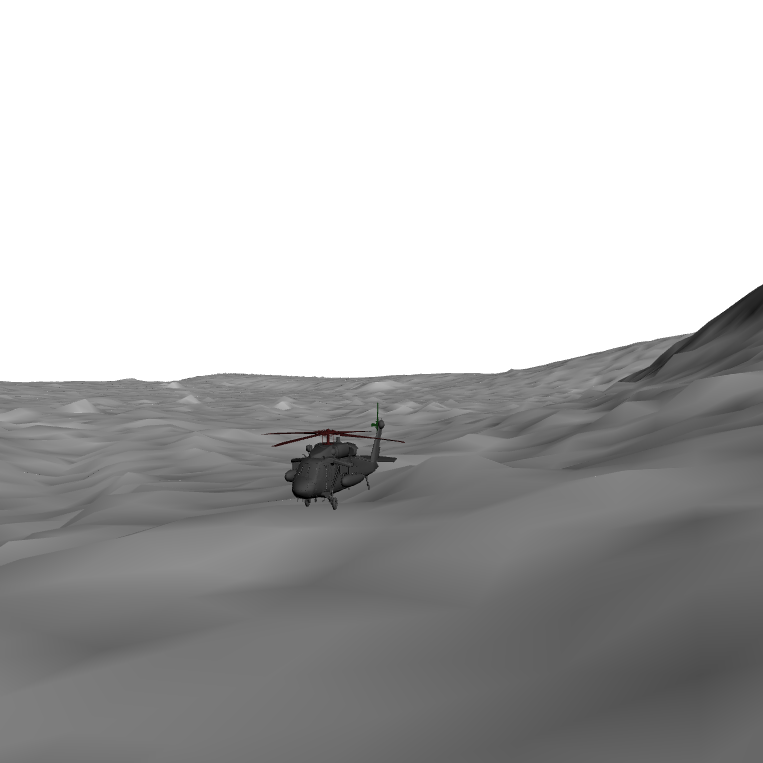
\includegraphics[width=0.5\columnwidth]{chopper}
\caption{A helicopter on the moon}
\label{fig:chopper}
\end{figure}


\setcounter{section}{4}
\section{}
\subsection{}
In the following figures, the helicopter has been rotated a quarter turn, but clearly does not obey the laws of light, and the dark side of the helicopter stays dark even though it is supposedly lit from the correct direction.
\begin{figure}[H]
\centering
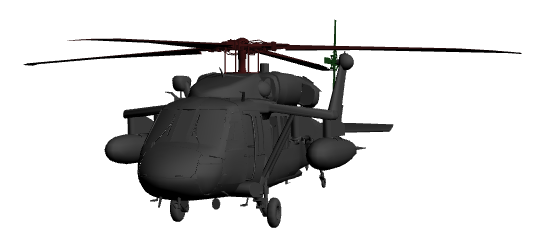
\includegraphics[width=0.5\columnwidth]{light-heli}
\caption{The bright side of the helicopter}
\label{fig:light-heli}
\end{figure}

\begin{figure}[H]
\centering
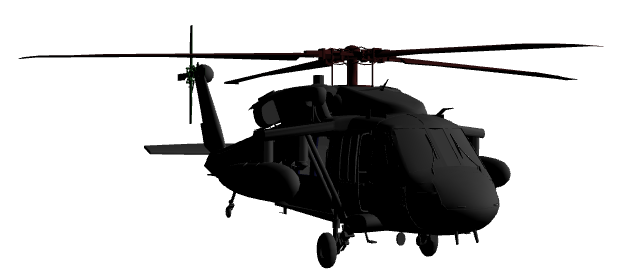
\includegraphics[width=0.5\columnwidth]{dark-heli}
\caption{The dark side of the helicopter}
\label{fig:dark-heli}
\end{figure}

The issue becomes even clearer when rendering multiple helicopters simultaneously as faces that point the same way get completely different shading. Observe how the two leftmost helicopters in figure \ref{fig:darkest} both have surfaces facing the camera, but one is lit and one is dark.

\begin{figure}[H]
\centering
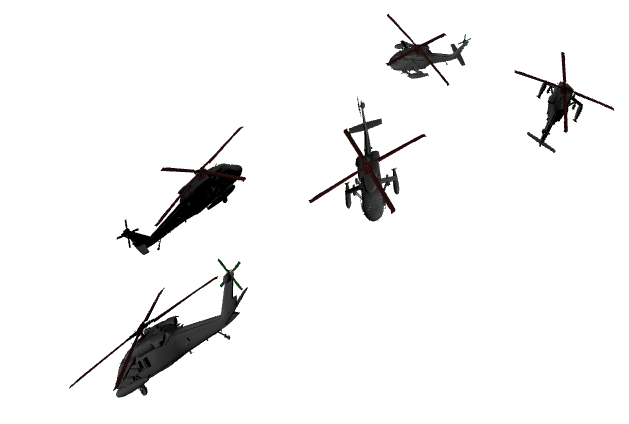
\includegraphics[width=0.5\columnwidth]{darkest-heli}
\caption{The two leftmost helicopters have very different shading}
\label{fig:darkest}
\end{figure}


\setcounter{section}{6}
\section{}
\setcounter{subsection}{1}
\subsection{Controllable Helicopter}
We add another helicopter above the five figure-8 helicopters that we wish to control. The dynamics of this helicopter is a grossly simplified kind of helicopter dynamics, with no special motion whatsoever. You can however control it just fine using wasd.

\begin{center}
\begin{tabular}{ |l|l| }
\hline
w & forward\\
a & rotate left\\
s & backward\\
d & rotate right\\
space & up\\
shift & down\\
c & toggle control\\
\hline
\end{tabular}
\end{center}

\subsection{Chase Camera}
Implementing the controllable helicopter without also implementing a chase camera was simply not acceptable, and so it had to be done. As with the helicopter, the chase camera is also done in a simple barely-work fashion. The camera needs some sort of control law to smoothly bring it to its target and the major simplification in this case is that control of each coordinate, x, y and z are decoupled, i.e. x-control depends only on x, y depends only on y and so on. The control laws we then opted for were the following
\begin{align*}
x_{k+1} = x_k - v(x_k - \text{sgn}(x_k - r_k)R - r_k),
\end{align*}
where $x_k$ and $r_k$ respectively denote the given coordinate of the camera and the reference (the helicopter), $v$ denotes the camera "speed" gain and $R$ denotes the wanted chase radius. This law is used for both the x and the z coordinate, but for y we omit the sign function to ensure that the helicopter is always chased from above. The keen eye will notice that this doesn't really keep the camera in a circle around its target, but rather in a square-like shape, in fact it will move according to figure \ref{fig:quiver} below.
\begin{figure}[H]
\centering
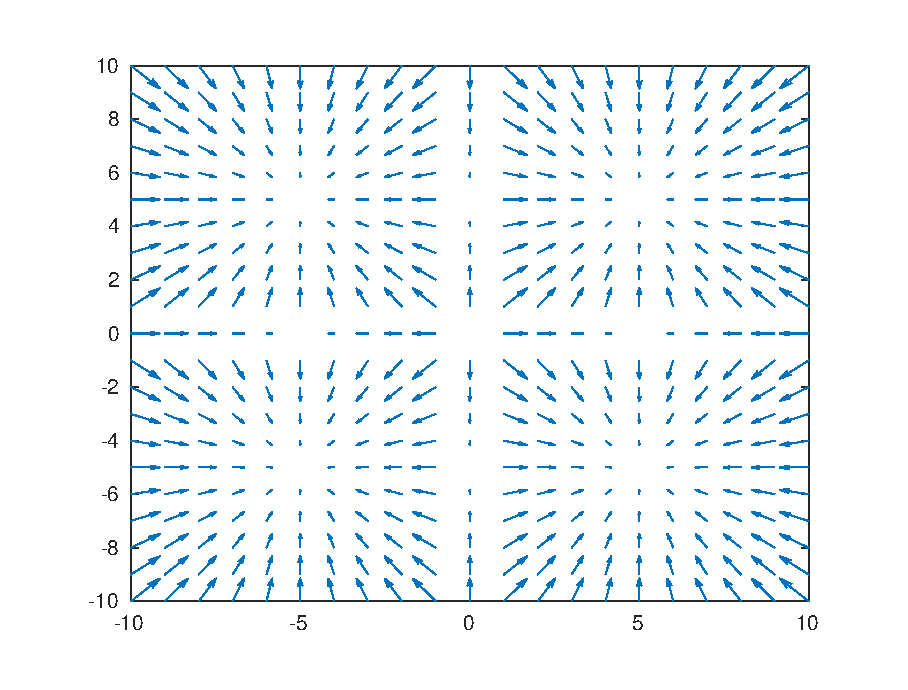
\includegraphics[width=0.69\columnwidth]{quiver.eps}
\caption{Quiver plot of chase camera dynamics}
\label{fig:quiver}
\end{figure}
We see that the camera will tend towards one of four stable points around the helicopter.

Finally, once the camera motion was in place, making the camera look at its target was as simple as using the opengl \texttt{lookAt} function.

Use the \texttt{c}-key to toggle between chase camera/helicopter control and the regular free-moving camera.

\setcounter{subsection}{5}
\subsection{}
You wanted to be amazed, so here you go. I proudly present \textit{deepfry-shading}, or in other words, what happens when the \textit{uninitialized} output color vector is used to color the scene.
\begin{figure}[H]
\centering
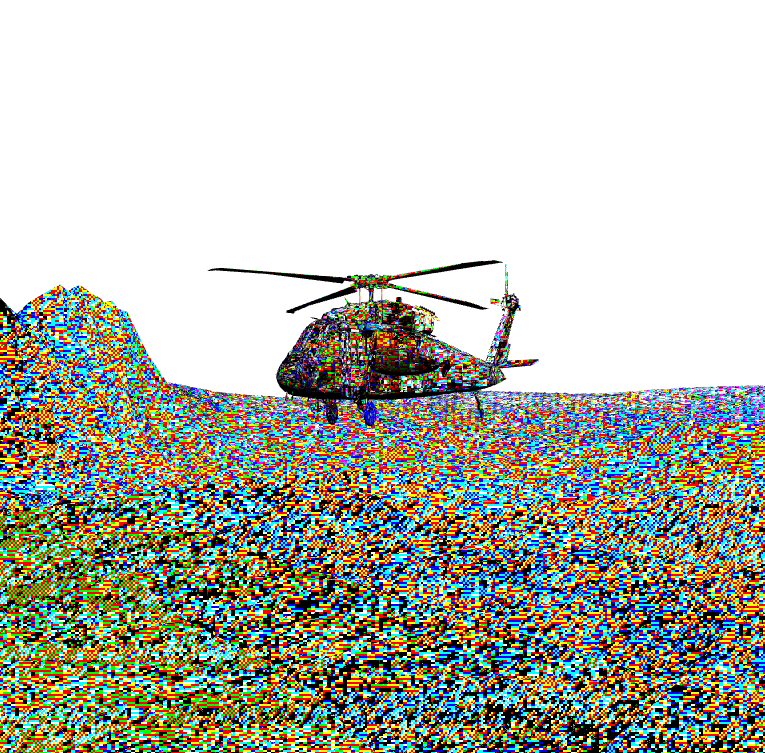
\includegraphics[width=0.7\columnwidth]{deepfry}
\caption{Deepfried Helicopter}
\label{fig:deepfry}
\end{figure}

\end{multicols}
\end{document}
